\section{基本要求一：编译系统的完整工作过程}
\label{sec:toolchain}
\subsection{实验程序与完整编译流程}
\label{sec:toolchain-flow}
主程序计算
\[
 S(n)=\sum_{i=0}^{n-1}(-1)^i(3i+5),\qquad R(n)=S(n)+11,\quad 0\leq n\leq20.
\]
静态函数 \texttt{scale\_and\_bias} 用于观察同单元内联，独立 \path{bonus.c} 中的 \texttt{add\_bonus} 则形成跨文件链接依赖。由相邻两项相消得到预期结果 $S(2k)=-3k$、$S(2k+1)=3k+5$。GCC/Clang 各有 O0、O2、O2-g 三组，每组七个有效输入和三个错误输入，共完成 \textbf{60/60} 次运行测试，输出与退出状态均符合预期。

所有编译器和优化配置均使用相同的两个源文件及同一组输入，以便对照阶段产物和运行结果；O0、O2 与 O2-g 的差异分别用于观察优化和调试信息对产物的影响。

从 C 源程序到可执行文件，需要依次完成预处理、编译、汇编和链接。图\ref{fig:toolchain-flow} 按产物类型标出这些处理的先后关系；保存各阶段产物后，可以分别观察文本变换、目标指令生成与外部符号解析。
\begin{figure}[H]
\centering
\begin{tikzpicture}[
  artifact/.style={draw=nkuPurple,fill=softBlue,rounded corners,align=center,
    text width=1.55cm,minimum height=1.1cm,font=\small},
  process/.style={align=center,font=\scriptsize},
  node distance=1.55cm,>=Latex]
\node[artifact] (tcsource) {源程序\\\texttt{.c}};
\node[artifact,right=of tcsource] (tcpre) {预处理文件\\\texttt{.i}};
\node[artifact,right=of tcpre] (tcasm) {汇编程序\\\texttt{.s}};
\node[artifact,right=of tcasm] (tcobj) {可重定位\\目标文件\\\texttt{.o}};
\node[artifact,right=of tcobj] (tcexe) {可执行文件\\ELF};
\draw[->] (tcsource) -- node[above,process]{预处理器\\\texttt{-E}} (tcpre);
\draw[->] (tcpre) -- node[above,process]{编译器\\\texttt{-S}} (tcasm);
\draw[->] (tcasm) -- node[above,process]{汇编器\\\texttt{-c}} (tcobj);
\draw[->] (tcobj) -- node[above,process]{链接器} (tcexe);
\node[below=0.35cm of tcexe,align=center,font=\scriptsize] (tclib) {其他目标文件\\与运行库};
\draw[->] (tclib.west) -| ([xshift=-0.7cm]tcexe.west);
\end{tikzpicture}
\caption{C 程序的完整编译流程；箭头表示处理阶段，方框表示输入或输出产物。}
\label{fig:toolchain-flow}
\end{figure}

\texttt{-E/-S/-c} 分别停止在预处理文本、汇编文本和目标文件阶段\cite{gcc}，但并非每个理论阶段都对应独立文件。本节机器码为本机 x86\_64，下一节手写汇编统一为 RISC-V。

下面以 Clang O0 展示实验中的分阶段调用。命令在 WSL 工程根目录执行；\texttt{F} 表示公共编译选项，\texttt{P} 表示该组产物目录，文件路径按工程根目录写为相对路径。\texttt{main.c} 和 \texttt{bonus.c} 分别生成目标文件，最后共同参与链接：
\begin{lstlisting}[language=bash,caption={Clang O0 的预处理、编译、汇编与链接命令},label={lst:toolchain-commands}]
F='-std=c11 -Wall -Wextra -Werror -march=x86-64 -mtune=generic -fno-pie -O0'
P=artifacts/toolchain/clang_O0
clang-14 $F -E src/toolchain/main.c -o "$P/main.i"
clang-14 $F -E src/toolchain/bonus.c -o "$P/bonus.i"
clang-14 $F -S "$P/main.i" -o "$P/main.s"
clang-14 $F -S "$P/bonus.i" -o "$P/bonus.s"
clang-14 -c "$P/main.s" -o "$P/main.o"
clang-14 -c "$P/bonus.s" -o "$P/bonus.o"
clang-14 -no-pie "$P/main.o" "$P/bonus.o" -Wl,-Map,"$P/link.map" -o "$P/demo"
\end{lstlisting}

GCC 采用同样的分阶段方式。\texttt{-S} 在这里读取已预处理的 \texttt{.i}，\texttt{-c} 则读取 \texttt{.s} 并停止于 \texttt{.o}；链接调用由编译器驱动组织目标文件、系统启动代码与运行库。不同优化配置的结果集中在\ref{sec:toolchain-optimization}节比较。

\subsection{预处理器做了什么？}
\label{sec:toolchain-preprocessor}
预处理器负责宏展开、头文件包含、条件编译以及其他预处理指令。它主要完成源代码级文本变换，不会对普通程序表达式求值，也不会生成机器代码；\texttt{\#if} 中的预处理条件表达式则由预处理器判断。\texttt{main.c} 包含 \texttt{stdio.h} 和 \texttt{demo.h}；后者通过头文件保护控制重复包含，并定义 \texttt{SCALE}、\texttt{BIAS} 等宏。

预处理将宏展开为 \texttt{3*x+(12-7)}，尚未计算括号；O0 IR 已使用常数 5。这说明宏替换只把宏定义中的文本放到使用位置，而常量表达式的处理发生在后续前端与 IR 生成过程中。\texttt{.i} 中还包含头文件展开后的声明，供编译器理解函数调用及其类型。

\subsection{编译器做了什么？}
\label{sec:toolchain-compiler}
编译器负责理解源程序的词法、语法和语义，建立中间表示，执行分析和优化，最终产生目标体系结构相关代码。本实验以 \texttt{.s} 为编译阶段的输出，并另行导出 AST 和 LLVM IR 观察中间结构。AST 中的 \texttt{ForStmt/IfStmt}、IR 中的基本块和 \texttt{br}、汇编中的指令及 ELF 中的重定位，分别反映前端结构处理、中间表示、代码生成和链接的结果。

\subsubsection{词法分析}
\label{sec:toolchain-lexing}
词法分析把字符流划分为 token，包括关键字、标识符、整数或浮点常量、运算符和分隔符。例如 \texttt{int sum = 0;} 中，\texttt{int} 是关键字，\texttt{sum} 是标识符，\texttt{0} 是整数常量，\texttt{=} 和 \texttt{;} 分别承担赋值与语句分隔功能。本实验未单独导出 token 序列，以下使用已保存的 AST 与 IR 观察前端处理结果。

\subsubsection{语法分析}
\label{sec:toolchain-parsing}
语法分析按语言文法将 token 组织为抽象语法树。\texttt{alternating\_sum} 的 AST 中，\texttt{ForStmt} 对应循环的初始化、条件、增量和循环体，\texttt{IfStmt} 对应奇偶判断与两个累计分支；\texttt{CallExpr} 对应辅助函数调用。这些节点把源代码的语句嵌套关系表达为树形结构。

\subsubsection{语义分析}
\label{sec:toolchain-semantics}
语义分析在语法结构上检查类型、符号绑定、作用域、函数参数及其他合法性约束。本实验主要通过 AST 与后续 IR 结果间接观察语义分析结果，而非将语义分析器本身作为单独程序输出。AST 中的 \texttt{DeclRefExpr} 关联变量或函数声明，\texttt{ImplicitCastExpr} 表示左值到值等隐式转换；后续 IR 中的 \texttt{i32} 参数、整数运算与返回值反映其类型结果。宏中的 \texttt{12-7} 在 O0 IR 中表现为常数 5，说明即使未启用 O2，前端仍需完成常量表达式处理。

\subsubsection{LLVM IR 生成}
\label{sec:toolchain-ir-generation}
中间代码生成将 AST 中的程序结构转换为 LLVM IR。O0 的 \texttt{alternating\_sum} 用 \texttt{alloca} 为局部状态分配存储位置，用 \texttt{load/store} 读写变量，用 \texttt{call} 表示 \texttt{scale\_and\_bias} 调用。循环和奇偶判断划分为基本块，\texttt{icmp} 产生条件，\texttt{br} 将各块连接起来，\texttt{ret} 返回累计结果。这里已经表达了程序的控制流与数据操作，但尚未选定每条操作使用哪个 x86 寄存器。

\subsubsection{中间代码优化}
\label{sec:toolchain-ir-optimization}
优化在保留程序语义的前提下变换中间表示。本实验的 O2 结果包含函数内联、以 \texttt{select} 表达奇偶项选择、\texttt{phi} 表达循环累计状态，以及整数归约的向量化、展开和标量尾部处理。\ref{sec:toolchain-optimization}节结合 pass 前后 IR、optimization remark 与产物大小完整分析这些变化。

\subsubsection{目标代码生成}
\label{sec:toolchain-code-generation}
目标代码生成把 LLVM IR 中的操作映射到目标指令，通过指令选择、寄存器分配等步骤输出汇编。Clang O0 的 \texttt{main.s} 中，辅助函数计算使用 \texttt{imull/addl}，分支使用 \texttt{jge/jne} 等跳转，调用使用 \texttt{callq}；汇编标签对应基本块和分支目标。局部 \texttt{sum} 的栈访问保留了 O0 对局部状态的直接实现。上述汇编尚含符号引用，需经汇编与链接生成可执行程序。

\subsection{汇编器做了什么？}
\label{sec:toolchain-assembler}
汇编器把指令助记符、寄存器、地址表达式和 label 转换为机器编码，并生成可重定位目标文件 \texttt{.o}。目标文件同时包含 section、symbol table 和 relocation information：section 组织代码与数据，符号表描述定义及外部引用，重定位信息记录需要链接器修正的地址或位移。

本实验通过 \texttt{clang-14 -c main.s -o main.o} 汇编阶段调用生成 \texttt{main.o}，并用 \texttt{readelf -hSWsrd} 与 \texttt{objdump -drwC -Mintel} 检查其 ELF 结构及指令编码。其文件类型为可重定位 ELF，\texttt{.text} 保存机器码，\texttt{.rodata.str1.1} 保存字符串。静态辅助函数为 LOCAL，\texttt{main} 为 GLOBAL，\texttt{add\_bonus/printf} 则是尚未定义的 UND 符号；\texttt{.rela.text} 为后续链接保存重定位项。

\subsection{链接器做了什么？}
\label{sec:toolchain-linker}
链接器合并多个目标文件，完成符号解析、重定位和地址布局，连接所需运行库，生成最终可执行文件。对每个外部引用，它需要在其他目标文件或库中找到定义，并依据重定位类型修正对应位置。

\texttt{main.o} 引用 \texttt{add\_bonus}，\texttt{bonus.o} 提供其定义。省略 \texttt{bonus.o} 时，链接报 \texttt{undefined reference to add\_bonus}；补回后成功，这对应符号解析是否找到定义的两种结果。\texttt{printf} 通过动态链接信息及 PLT/GOT 关联 libc 中的实现。表\ref{tab:link} 将目标文件中的符号、重定位与这项链接负对照放在一起，说明汇编器留下的信息如何被链接阶段使用。

\begin{table}[H]
\centering\small
\caption{Clang O0 的目标文件与链接分析}
\label{tab:link}
\begin{tabularx}{\textwidth}{L{2.5cm}Y}
\toprule\rowcolor{tableHead}观察项 & 结果及含义 \\
\midrule
代码与符号 & \texttt{.text} 存机器码，\texttt{.rodata.str1.1} 存字符串；静态辅助函数为 LOCAL，\texttt{main} 为 GLOBAL，\texttt{add\_bonus/printf} 为 UND。局部 \texttt{sum} 在栈上。\\
重定位与解析 & \texttt{.rela.text} 的 12 项中包含两者的 \texttt{R\_X86\_64\_PLT32} 引用；\texttt{bonus.o} 提供前者定义，后者通过动态链接信息与 PLT/GOT 在运行时绑定 libc 中的实现。\\
链接负对照 & 省略 \texttt{bonus.o} 后报 \texttt{undefined reference to add\_bonus}，补回后成功。该预期失败不计入程序运行通过数。\\
\bottomrule
\end{tabularx}
\end{table}

\subsection{各阶段输入、输出与实验产物总结}
\label{sec:toolchain-stage-summary}
表\ref{tab:toolchain-stages} 按输入、命令、功能和输出汇总完整工具链，便于对照各阶段职责。这里的编译器驱动组织各阶段调用；AST 与 LLVM IR 是为观察编译器内部结构而额外导出的中间结果。
\begin{table}[H]
\centering\small
\setlength{\tabcolsep}{3pt}
\caption{编译系统各阶段的输入、输出与观察结果}
\label{tab:toolchain-stages}
\begin{tabularx}{\textwidth}{L{1.25cm}L{1.45cm}L{2.25cm}L{2.45cm}L{1.65cm}Y}
\toprule\rowcolor{tableHead}阶段 & 输入 & 实际命令 & 主要功能 & 输出 & 本实验观察结果 \\
\midrule
预处理 & \texttt{.c} 与头文件 & \makecell[l]{\texttt{clang-14}\\\texttt{-E}} & 宏替换、包含头文件、条件编译 & \texttt{main.i}、\texttt{bonus.i} & 展开为 \texttt{3*x+(12-7)}，括号未求值。\\
编译 & 预处理后的 \texttt{.i}；导出 IR 时输入 \texttt{.c} & \makecell[l]{\texttt{clang-14}\\\texttt{-S}；另用\\\texttt{-S}\\\texttt{-emit-llvm}} & 前端分析、IR 生成与优化、目标代码生成 & \texttt{.s}；另有 AST、\texttt{.ll} & AST 含 \texttt{ForStmt/IfStmt}，IR 含基本块与 \texttt{br}，汇编含目标指令。\\
汇编 & \texttt{main.s}、\texttt{bonus.s} & \makecell[l]{\texttt{clang-14}\\\texttt{-c}} & 指令编码，组织节、符号及重定位项 & 可重定位 \texttt{.o} & \texttt{.text}、LOCAL/GLOBAL/UND、\texttt{.rela.text}。\\
链接 & 两个 \texttt{.o} 与系统运行库 & \makecell[l]{\texttt{clang-14}\\\texttt{-no-pie}\\\texttt{main.o}\\\texttt{bonus.o}} & 符号解析、重定位、地址布局与运行库连接 & 可执行 ELF \texttt{demo} 与 \texttt{link.map} & \texttt{add\_bonus} 由 \texttt{bonus.o} 解析，\texttt{printf} 动态关联 libc；缺少前者时失败。\\
\bottomrule
\end{tabularx}
\end{table}

\subsection{补充探索：优化策略与源程序变化对编译结果的影响}
\label{sec:toolchain-optimization}
完整流程说明每个阶段负责什么；下面比较 O0、O2 与 O2-g，解释同一程序在优化配置变化后为何产生不同的 IR、指令结构与文件大小。
在这些基线分析之后，进一步通过向量化与展开开关、GCC 优化级别以及辅助函数 noinline 微扰，检验优化现象及其阶段依赖；所有新增结果均独立构建、测量与验证。

\subsubsection{从循环依赖到整数归约}
\label{sec:toolchain-reduction}
O0 IR 仍以 \texttt{alloca/load/store} 表示局部状态，并在循环内调用辅助函数。内联诊断显示辅助函数被内联；\texttt{LoopVectorizePass} 前的 IR 中，奇偶分支已成为选择带符号项的 \texttt{select}，累计和成为下面的 SSA 递推（摘录省去位置元数据）：
\begin{lstlisting}[caption={向量化前的归约环；数值名来自 pass 前 IR}]
%9 = phi i32 [ %17, %8 ], [ 0, %3 ]
; %16 chooses +(3*i+5) or -(3*i+5)
%16 = select i1 %14, i32 %12, i32 %15
%17 = add i32 %16, %9
\end{lstlisting}
这里 \texttt{\%9} 依赖上一轮的 \texttt{\%17}，因此循环存在跨迭代依赖；\texttt{i} 则是规律递增的归纳变量。关键在于每项只依赖自己的索引，内联后没有待保留的函数副作用，累计状态仅沿“\texttt{phi}$\to$\texttt{add}$\to$\texttt{phi}”回传。它是可分组求和的整数归约，而非必须保持逐轮处理顺序的一般递推，与 LLVM 的 reduction 识别机制一致\cite{llvmvector14}。该分析针对声明输入域内不溢出的整数求和；C 有符号溢出和浮点求和的舍入顺序不在此结论范围内。

向量化诊断采用 Clang 14 和 \texttt{-O2 -march=x86-64 -mtune=generic -fno-pie} 等选项，并启用 \texttt{-Rpass}、\texttt{-Rpass-missed}、\texttt{-Rpass-analysis} 的 \texttt{loop-vectorize} 过滤及 YAML 记录\cite{clangremarks14}。同一源代码行对应两个不同的函数上下文：
\begin{table}[H]
\centering\small
\caption{optimization remarks 区分的两个循环上下文}
\label{tab:vector-remarks}
\begin{tabularx}{\textwidth}{L{3.1cm}L{1.1cm}L{1.1cm}Y}
\toprule\rowcolor{tableHead}所在函数 & 宽度 & 交错数 & 诊断及最终 IR \\
\midrule
\texttt{alternating\_sum} & 4 & 2 & 两个四通道累计器；每轮覆盖八个源迭代。\\
\texttt{main} 内联副本 & 4 & 1 & 明确报告交错无收益；另有 \texttt{FullyUnrolled}、次数 5 的记录，最终成为常量向量选择及尾部路径。\\
\bottomrule
\end{tabularx}
\end{table}
诊断没有报告 loop-vectorize 的 missed 项。启用记录选项后，IR 与汇编含有 \texttt{!dbg/.loc} 位置元数据；剔除元数据后的函数体与未启用记录时相同，\texttt{main.o} 代码段内容也相同。

\subsubsection{向量通道、尾部与展开}
\label{sec:toolchain-vector-tail}
独立函数的 \texttt{<4 x i32>} 是四个 32 位整数通道，不是四个线程。

设带符号项为 $t_i=(-1)^i(3i+5)$，第 $k$ 个向量循环中，两组累计器的第 $j$ 通道分别累加 $t_{8k+j}$ 与 $t_{8k+4+j}$（$0\leq j<4$）。这是宽度 4、交错数 2 对应的部分展开；最终 IR 中第二组常数 17 来自 $3(i+4)+5=3i+17$，对应索引偏移 4 的同一计算。奇偶条件按通道变成比较及 \texttt{select}，两个累计向量先逐通道相加，再由 \texttt{llvm.vector.reduce.add.v4i32} 将四通道横向求和为一个 i32\cite{llvm}；汇编的 \texttt{paddd/pshufd} 对应这些操作。

循环次数由输入决定，未必被八整除。pass 后的 IR 先计算 $m=n-(n\bmod8)$；最终 IR 将其简化为 \texttt{n \& -8}。$n<8$ 时直接走标量路径，否则向量段处理前 $m$ 项，标量尾部从归约所得的部分和继续处理 $m$ 到 $n-1$，且尾部未再次向量化。内联到 \texttt{main} 后，已知 $n\le20$ 的上下文使用宽度 4、交错数 1；最多五个向量批次的循环被完全展开，与最终按批次数选择预计算向量的结构一致，标量尾循环仍保留。

为直接核验上述尾部路径，另在原 Clang O2 可执行程序及直接调用独立函数的合法入口上执行 $n=7,8,9,15,16,17$。独立入口通过链接器 \texttt{--wrap=main} 选择测试函数，所链接的 \texttt{alternating\_sum} 299 字节机器码与原程序逐字节一致；\texttt{main} 上下文则直接运行原程序。GDB 在反汇编定位的向量循环头、标量循环头和 \texttt{main} 归约块设置断点，实际命中次数见表\ref{tab:vector-boundaries}，不以最终输出相同推断路径。

\begin{table}[H]
\centering\small
\caption{Clang O2 边界输入的实际断点命中次数}
\label{tab:vector-boundaries}
\begin{tabularx}{\textwidth}{L{0.8cm}Y Y Y Y}
\toprule\rowcolor{tableHead}
$n$ & 独立函数向量循环 & 独立函数标量迭代 & \texttt{main} 归约块 & \texttt{main} 标量迭代 \\
\midrule
7  & 0 & 7 & 1 & 3 \\
8  & 1 & 0 & 1 & 0 \\
9  & 1 & 1 & 1 & 1 \\
15 & 1 & 7 & 1 & 3 \\
16 & 2 & 0 & 1 & 0 \\
17 & 2 & 1 & 1 & 1 \\
\bottomrule
\end{tabularx}
\end{table}

独立函数的向量批次与标量迭代分别为 $\lfloor n/8\rfloor$ 与 $n\bmod8$，包括小于阈值时的纯标量路径；$n=17$ 的日志实际记录两次向量头命中，以及从索引 16 开始的一次标量迭代。\texttt{main} 已无对应向量回边，其归约块一次命中表示展开后选定向量的归约，不能解释为一个八元素批次；其尾部次数为 $n\bmod4$。特别是 $n=7$，\texttt{main} 已执行常量向量归约，随后处理索引 4、5、6，而独立函数执行七次标量迭代。运行 \texttt{main} 时独立函数入口均未命中，进一步区分了两个上下文。六个输入、两种入口的输出、stderr 与退出状态为 12/12 通过，路径计数也为 12/12 通过；独立数值预期仍由配对求和公式计算。详细地址、断点脚本、寄存器命中日志及机器码一致性证据保存在 \path{artifacts/toolchain/extended_exploration/boundary/}。这些证据验证了当前二进制的边界处理，不代表其他配置或更大输入域。

\subsubsection{Clang 向量化与循环展开的受控实验}
\label{sec:toolchain-clang-controlled}
为检验 Clang O2 代码增长与向量化、循环展开之间的关系，本轮固定原始 \texttt{main.c}、\texttt{bonus.c} 和 \texttt{demo.h}、Clang 14.0.0、通用 x86-64 目标及原有公共选项，构建四组配置：A 为 \texttt{-O2}；B 在 A 上添加 \texttt{-fno-vectorize -fno-slp-vectorize}；C 添加 \texttt{-fno-unroll-loops}；D 同时添加上述三个关闭选项。各组仍分别预处理、编译、汇编并以 \texttt{-no-pie} 链接，没有启用 LTO。新增 A 的可执行文件 \texttt{.text} 与旧 Clang O2 逐字节一致，因此表\ref{tab:clang-controlled} 中的 A 是重新构建并测量的对照，而非直接抄录旧值。

\begin{table}[H]
\centering\footnotesize
\setlength{\tabcolsep}{3pt}
\caption{Clang 四组控制实验的实际结果；BB 按独立函数／\texttt{main} 给出}
\label{tab:clang-controlled}
\begin{tabularx}{\textwidth}{L{0.45cm}L{1.55cm}L{2.15cm}Y L{1.05cm}L{0.95cm}L{0.9cm}L{1.0cm}}
\toprule\rowcolor{tableHead}
组 & 向量／展开开关 & 实际向量化 VF/IC & 实际展开 & IR BB & \texttt{.text} B & 指令 & 测试 \\
\midrule
A & 开／开 & 4/2；4/1 & \texttt{main} 完全展开 5 次 & 8/16 & 868 & 154 & 10/10 \\
B & 关／开 & 两者均无 & 两者标量循环均展开 2 次 & 7/12 & 596 & 105 & 10/10 \\
C & 开／关 & 4/1；4/1 & 无成功展开记录，向量回边保留 & 8/13 & 836 & 150 & 10/10 \\
D & 关／关 & 两者均无 & 无成功展开记录，标量回边保留 & 3/8 & 500 & 76 & 10/10 \\
\bottomrule
\end{tabularx}
\end{table}

表中“开／关”表示请求的配置，“实际向量化”与“实际展开”两列观察来自实际 IR 与 optimization remarks。BB 是最终 LLVM IR 的基本块数，含隐式入口块；\texttt{.text} 是可执行文件代码节，含启动代码；指令数继续按 \texttt{main.o} 的反汇编指令行统计，含对齐 nop。分支指令只计 \texttt{j*} 与 \texttt{loop*}，不计调用和返回，A/B/C/D 分别为 18/14/14/8 条。这些统计对象不同，不能把 IR 的块数直接当成机器分支数。

B、D 的最终函数体均没有整数向量类型或 \texttt{llvm.vector.reduce.add} 调用，汇编也没有对应 SIMD 主体，因而关闭向量化的实际效果得到核验。但归约没有消失：D 仍保留标量 \texttt{phi}、带符号项选择及回传累计值。B 的诊断在两个上下文均报告 \texttt{PartialUnrolled}、次数 2；其独立函数每次回边将索引加 2，先后累计一正一负两项，并对奇数项数保留收尾处理。D 则只保留逐项标量循环。下面摘录 D 的真实归约链，省略与该链无关的指令：
\begin{lstlisting}[caption={同时关闭向量化与展开后仍存在的标量归约}]
%6 = phi i32 [ %14, %5 ], [ 0, %1 ]
; %13 selects the signed scalar term
%13 = select i1 %11, i32 %9, i32 %12
%14 = add i32 %13, %6
\end{lstlisting}

C 说明关闭展开还会改变向量循环的交错策略。独立函数的诊断明确报告 \texttt{InterleavingBeneficialButDisabled}，VF 仍为 4，IC 从 2 降至 1；最终 IR 每次索引增加 4，而非 A 的 8，并继续使用横向归约与标量尾部。\texttt{main} 也保留四通道向量循环的 \texttt{phi} 和回边，不再出现 A 的五次完全展开记录。这里没有观察到另一个成功的 loop-unroll 记录，但四通道 SIMD 与常量表达式仍存在，不能将关闭展开解释为取消全部并行通道或常量化。

按 \texttt{nm -S} 的符号大小，独立函数 A/B/C/D 分别为 299/96/219/59 B，\texttt{main} 为 315/244/367/192 B。C 的独立函数缩小，\texttt{main} 却增大：A 的有界向量循环展开后可进一步形成常量向量选择，C 保留运行时向量索引、算术与回边。该结构差异能解释为何关闭展开未必使每个函数都缩小；函数大小也不含函数间对齐填充，不能与可执行文件 \texttt{.text} 混为同一指标。

四组数据还可检验交互。A$-$B、A$-$C、A$-$D 分别减少 272/32/368 B，及 49/4/78 条指令。联合减少量比两项单独减少量之和多 64 B、25 条。若以 $y$ 表示同口径指标，则
\[
 I=y_A-y_B-y_C+y_D
   =\begin{cases}-64\ \mathrm{B},& y=\texttt{.text};\\-25,& y=\text{静态指令数}.\end{cases}
\]
有向量化时，关闭展开减少 32 B；没有向量化时则减少 96 B。这与 A 的向量交错及有界完全展开、B 的标量两次展开、C 的未展开向量循环、D 的单次标量循环相对应，说明两个配置因素共同改变了优化后 CFG 与指令结构。开关同时影响后续分析和变换，因此这些差值支持配置之间存在交互，不能当作某个 pass 的独立空间贡献。

四组均重新执行原有十类输入检查，以配对求和公式作为独立预期，逐项比较 stdout、stderr 与退出状态，合计 40/40。完整命令、源码 SHA256、IR、CFG、汇编、ELF、诊断和逐项结果保存在 \path{artifacts/toolchain/extended_exploration/configs/} 下的四个 Clang 配置目录；汇总指标见该实验目录的 \texttt{metrics.json/csv}。本实验只比较代码结构，不测量执行速度。

\subsubsection{GCC 优化级别与向量化配置比较}
\label{sec:toolchain-gcc-controlled}
Clang 的结果提示优化集合可能影响代码结构，但 GCC O2 没有启用向量化并不意味着显式开启后就一定成功。为区分“默认未开启”和“开启后识别失败”，使用实际版本 GCC 11.4.0，保持源程序、公共选项及链接依赖不变：A 为 \texttt{-O2}；B 为 \texttt{-O2 -ftree-loop-vectorize -ftree-slp-vectorize}；C 为 \texttt{-O3}；D 为 \texttt{-O3 -fno-tree-loop-vectorize -fno-tree-slp-vectorize}。逐组查询优化选项，并保留 \texttt{-fopt-info-vec-all} 与 GIMPLE 输出，B/C 另保存详细向量化分析。

\begin{table}[H]
\centering\footnotesize
\setlength{\tabcolsep}{3pt}
\caption{GCC 优化配置比较；四组均未实际产生循环向量化}
\label{tab:gcc-controlled}
\begin{tabularx}{\textwidth}{L{0.45cm}L{0.65cm}L{1.6cm}L{1.15cm}Y L{0.9cm}L{1.0cm}L{1.0cm}}
\toprule\rowcolor{tableHead}
组 & 级别 & 向量化选项 & 实际结果 & 诊断／结构 & 指令 & \texttt{.text} B & 测试 \\
\midrule
A & O2 & 默认关闭 & 无向量化 & 标量循环；\texttt{main} 保留函数调用 & 66 & 520 & 10/10 \\
B & O2 & 显式开启两类 & 无向量化 & 尝试后报不支持的 def-use 模式 & 66 & 520 & 10/10 \\
C & O3 & 默认开启 & 无向量化 & 独立及内联循环均失败；\texttt{main} 已内联 & 79 & 552 & 10/10 \\
D & O3 & 显式关闭两类 & 无向量化 & 标量内联循环；代码与 C 相同 & 79 & 552 & 10/10 \\
\bottomrule
\end{tabularx}
\end{table}

选项查询确认 B/C 的两类向量化均为 enabled，A/D 为 disabled；最终 GIMPLE 没有向量变量声明，目标循环反汇编也没有 SIMD 指令。B 的独立函数、C 的独立函数与 \texttt{main} 内联副本均报告 \texttt{unsupported use in stmt}。详细分析进一步把障碍定位到累计状态：分析 \texttt{sum} 的循环 PHI 后出现 \texttt{reduction used in loop} 和 \texttt{Unknown def-use cycle pattern}，随后将其使用识别为 unknown，未生成向量循环。外围 \texttt{scanf/fwrite} 的 memory-clobber 诊断也被保留，但不能将其误作这个算术循环失败的原因。

GCC 的最终 GIMPLE 仍将累计值用于条件两侧的加法与减法，再由 PHI 合并；例如 B 的对应片段为：
\begin{lstlisting}[caption={GCC B 的标量累计状态；摘录保留原 GIMPLE 名称}]
# sum_6 = PHI <0(2), sum_24(6)>
; even branch
sum_23 = sum_6 + _17;
; odd branch
sum_22 = sum_6 - _17;
; merge and feed the next iteration
# sum_24 = PHI <sum_22(5), sum_23(4)>
\end{lstlisting}
与 Clang 在向量化前形成“先选带符号项、再统一加到累计值”的结构相比，两者暴露给向量分析的 def-use 形式不同。结合详细失败诊断，本例支持 GCC 11.4 在当前流水线中未接受该循环累计模式；它不能证明 GCC 普遍不支持整数归约，也不能说明只更改某一条 GIMPLE 就必然成功。

B 与 A 的全部目标代码节相同，可执行文件 \texttt{.text} 也相同；C 与 D 同样如此，故开启向量化在本例没有产生预期的向量代码。O3 仍带来另一项可见变化：A/B 的 \texttt{main} 保留 \texttt{alternating\_sum} 调用，C/D 则内联其标量循环。独立函数四组均为 51 B；\texttt{main} 从 195 B 变为 236 B，GIMPLE BB 从 6 变为 11，\texttt{main.o} 分支数从 7 变为 9。因而 O3 比 O2 多出的 32 B、13 条指令，与内联后的循环及布局变化相伴，不能归因于 SIMD 或直接等同于性能提升。

四组新增运行检查合计 40/40。GCC O2 显式向量化与 O3 都尝试了向量化并失败，但二者的内联和其他优化配置不同，最终产物并不相同；GCC O3 与 Clang O2 更不是严格匹配的 pass 流水线。默认优化集合解释了 GCC O2 没有发起同类变换的一部分背景，新增诊断则表明，仅统一“向量化开关”仍不足以统一两种编译器的结果。本轮没有数值化比较代价模型，也没有性能测量。详细证据位于四个 GCC 配置目录中的 \texttt{main.optinfo.txt}、\texttt{main.gimple}、B/C 的 \texttt{main.vect-details.gimple} 及反汇编。

\subsubsection{函数内联对后续循环优化的影响}
\label{sec:toolchain-noinline}
为检验内联是否改变后续循环优化机会，保持原始程序不变，在独立文件 \path{src/toolchain/variants/main_noinline.c} 中仅给 \texttt{scale\_and\_bias} 增加 \texttt{noinline} 属性。变体与原文件的差异检查确认只有该属性改变，函数仍计算 $3x+5$。两者均使用与 Clang A 相同的 O2 配置，结果见表\ref{tab:noinline-controlled}。

\begin{table}[H]
\centering\footnotesize
\setlength{\tabcolsep}{3pt}
\caption{Clang O2 原始程序与 noinline 微扰的对照}
\label{tab:noinline-controlled}
\begin{tabularx}{\textwidth}{L{1.4cm}L{1.5cm}L{1.35cm}Y L{1.0cm}L{0.85cm}L{1.0cm}}
\toprule\rowcolor{tableHead}
源码 & 循环内辅助调用 & 实际向量化 & 累计／归约结构 & \texttt{.text} B & 指令 & 测试 \\
\midrule
原始 & 无，已内联 & 两上下文均有 & 向量 PHI、向量相加及横向归约 & 868 & 154 & 10/10 \\
noinline & 两上下文均保留 & 两者均无 & 标量 PHI、选择及加法递推保留 & 532 & 91 & 10/10 \\
\bottomrule
\end{tabularx}
\end{table}

变体诊断明确报告辅助函数因 noinline 属性未被内联；其独立符号实际保留，大小为 7 B。\texttt{alternating\_sum} 本身仍被内联到 \texttt{main}，所以这组实验只禁止辅助函数内联，不能说所有内联都被关闭。最终 IR 在独立和内联上下文中各保留一个辅助调用点，机器汇编也保留相应 \texttt{call}。独立函数的关键片段如下：
\begin{lstlisting}[caption={noinline 变体的真实循环调用与标量累计链}]
%6 = phi i32 [ %13, %5 ], [ 0, %1 ]
%7 = phi i32 [ %14, %5 ], [ 0, %1 ]
%8 = tail call fastcc i32 @scale_and_bias(i32 noundef %7)
%11 = sub i32 0, %8
%12 = select i1 %10, i32 %8, i32 %11
%13 = add i32 %12, %6
\end{lstlisting}

\texttt{LoopVectorizePass} 的前后快照保留同一标量累计链与调用，没有产生向量循环或 \texttt{llvm.vector.reduce.add}；诊断在两个上下文均指出 \texttt{call instruction cannot be vectorized}。辅助函数仍被推导为 \texttt{readnone}，因此不能把失败简单归咎于它具有内存副作用。实际证据支持：本程序在该版本和配置下，内联将 $3i+5$ 暴露为循环内算术后能够向量化，而保留的辅助调用成为向量化诊断明确指出的障碍。标量归约形状并未消失；不过现有诊断未单独输出内部归约描述符的识别状态，不能仅凭 PHI/add 形状就声称向量器内部归约识别已经成功。

最终独立函数／\texttt{main} 的 LLVM BB 从 8/16 变为 3/8，符号大小从 299/315 B 变为 55/202 B，另保留 7 B 的辅助函数，\texttt{main.o} 分支数从 18 变为 9。代码缩小与向量入口、向量主体、归约和尾部等结构消失相对应，但调用开销、跨过程分析和后续优化机会也同时变化，不能把全部 336 B、63 条指令差异单独解释为一次内联 pass 的贡献，更不能据此评价运行速度。该变体新增检查为 10/10，连同前述八组共 90/90；边界路径检查另行统计，原有 60/60 基线记录不变。


\subsubsection{代码大小、调试信息与编译器差异}
\label{sec:toolchain-code-size}
图\ref{fig:metrics} 对照 GCC 与 Clang 在 O0/O2 下的代码结构指标，用于观察优化对静态代码空间的影响；随后结合 IR、配置和调试节说明这些变化的原因及解释范围。
\begin{figure}[H]
\centering
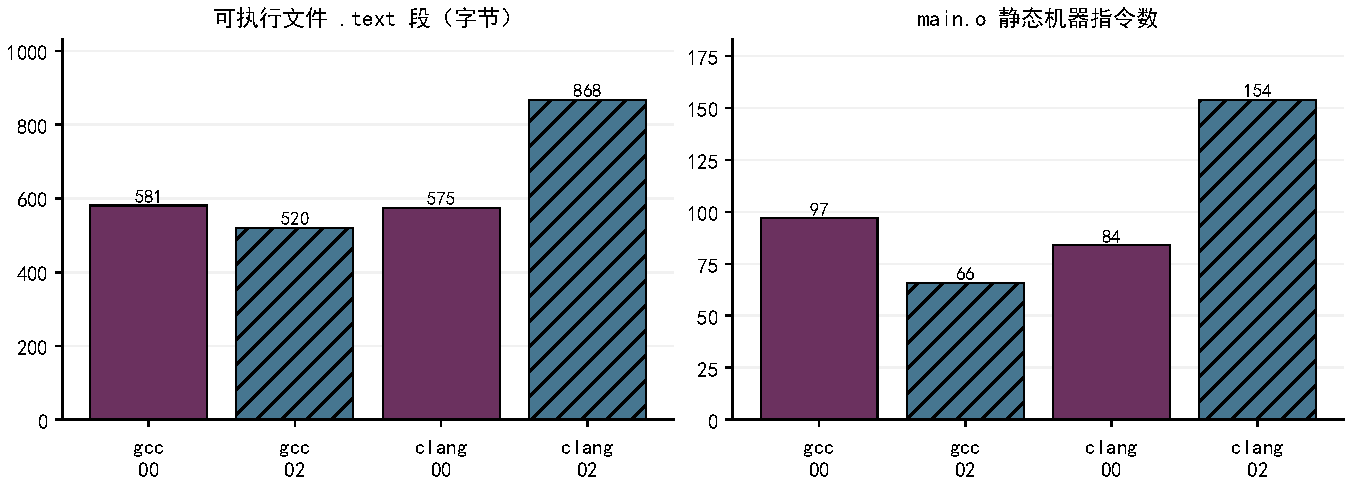
\includegraphics[width=\textwidth]{figures/toolchain_metrics.pdf}
\caption{代码结构指标：左图含链接启动代码，右图只计 \texttt{main.o} 的静态指令行（含填充 nop）。}
\label{fig:metrics}
\end{figure}
Clang O2 的 \texttt{.text} 从 575 B 增至 868 B，静态指令数从 84 增至 154。向量主体、横向归约、入口判断、标量尾部，以及内联后仍保留的独立函数定义都需要空间；\texttt{main} 的有界展开还改变了控制流。这些结构解释了为何优化可能增大代码。本文未进行逐 pass 消融，各结构对代码增量的单独贡献尚未量化。

GCC O2 的对应指标由 581 B/97 条降至 520 B/66 条，其循环改为从 5 开始每轮加 3 的归纳变量，分支变成 \texttt{testb/cmove}。同参数的 \texttt{gcc -Q --help=optimizers} 显示，\texttt{-ftree-loop-vectorize} 和 \texttt{-ftree-slp-vectorize} 均为 \texttt{[disabled]}；GCC 11.4 官方文档也将两者列为 O3 默认开启\cite{gccopt11}。本例的 GCC O2 配置没有启用这两类向量化优化；上述基线未包含 O3；本轮新增比较见\ref{sec:toolchain-gcc-controlled}节。

两者虽均指定通用 x86-64，完整优化流水线没有逐项对齐，GCC 默认安全选项及 O2 的 \texttt{\_FORTIFY\_SOURCE=2} 还改变系统头文件展开，其 O0 和 Clang O2 没有该宏。LLVM 的宽度与交错选择使用代价模型\cite{llvmvector14}；\texttt{main} 的诊断报告“交错无收益”，但没有给出该判断的数值成本。由于 GCC 与 Clang 在 O2 下启用的优化集合不同，代码大小差异不能直接用于评价两种编译器的优劣。本实验未测运行时间，不进行性能比较；文件大小和静态指令数量仅用于描述产物结构，不能据此推断执行时间。

O2 加 \texttt{-g} 后，GCC/Clang 可执行文件分别由 16216/16120 B 增至 21080/19136 B，\texttt{.debug*} 合计为 4239/2315 B。在本例中，两编译器各自 O2 与 O2-g 的整个 \texttt{.text} 内容相同，文件增长还含节表等元数据。跨翻译单元的 \texttt{add\_bonus} 调用仍保留，内联诊断说明其定义不可见；实验没有启用 LTO。

新增实验为上述解释补充了可量化的配置对照：Clang 的空间差异与向量主体、交错、展开及尾部结构共同变化，GCC O3 的差异则在未发生向量化的情况下伴随 \texttt{main} 内联。它们仍不构成逐 pass 的独立消融。诊断构建与普通构建逐一比较目标文件全部可执行代码节，GCC 同时检查 \texttt{.text} 与包含 \texttt{main} 的 \texttt{.text.startup}，九组均保持一致；只检查 GCC 的 \texttt{.text} 会漏掉 \texttt{main}，因此不能据其单节哈希断言整个目标代码相同。原有 60/60、新增配置 90/90 和边界入口 12/12 各自保留统计口径，均未转化为性能结论。
